\section{Product}
\label{sec:product}
\salespoint{} is intended as framework for point-of-sale applications.
The items for sale are called ``products'' and represented by instances of classes who implement the \code{Product} interface.
A general overview of the \salespoint{} products subsystem is given in Figure \ref{product_overview}.
To represent different kinds of products, \code{PersistentProduct} can be sub-classed; see Section \ref{jpa-types} for more information.
\code{PersistentProduct}s are aggregated by \code{PersistentCatalog} (see Section \ref{sec:catalog}).

\begin{figure}
	\centering
  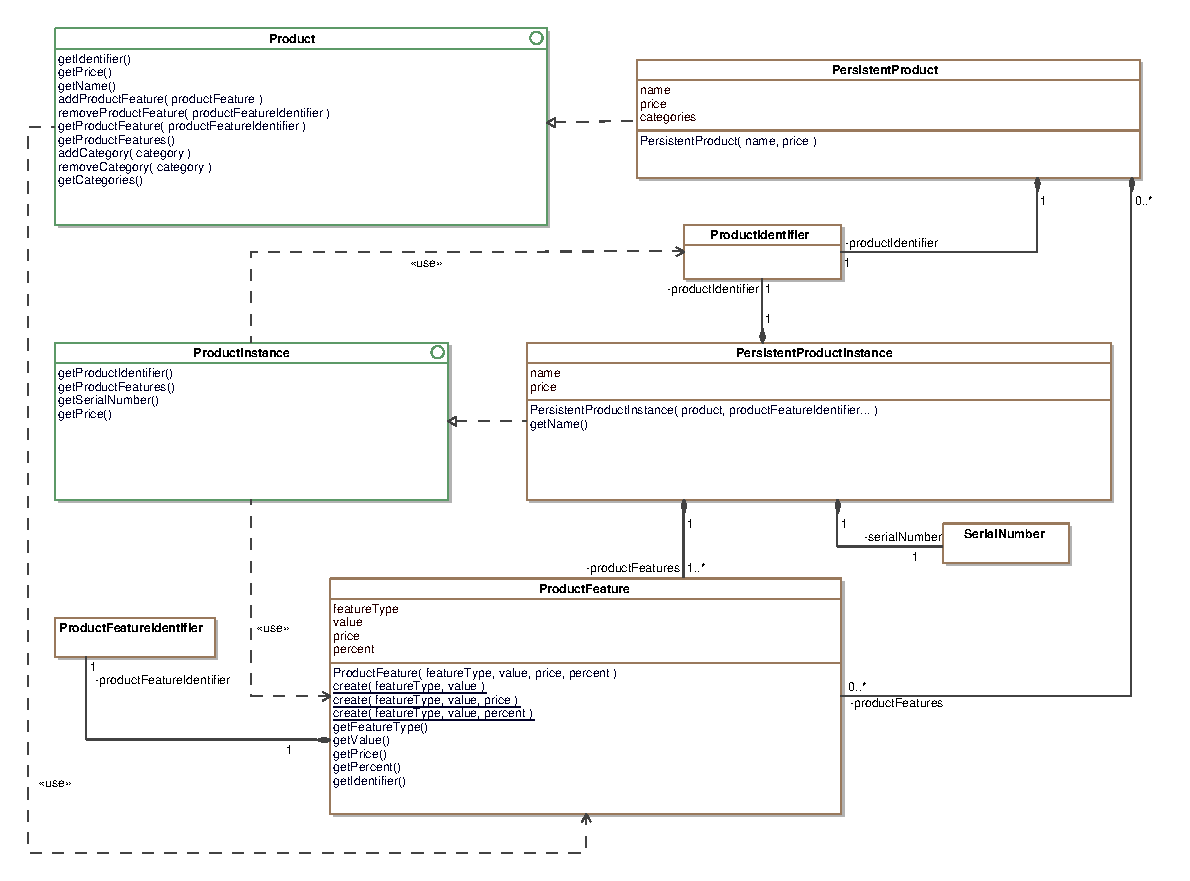
\includegraphics[width=1.0\textwidth]{images/Product_Overview.eps}
	\label{product_overview}
	\caption{Product - Class Overview}
\end{figure}

\code{Product}s are supposed to be an abstraction, like an item on display or a picture in a catalog.
\code{ProductInstance}s are used to represent the actual item you get, when you a buy a product.
\code{Product}s are identified using a \code{ProductIndentifier}, whereas \code{ProductInstance}s are identified by a \code{SerialNumber}.
\code{ProductInstance}s can be thought of as identifiable instances of a certain product, which are identical apart from their \code{SerialNumber}.
\\

To conviently handle products, which are essentially the same but differ in certain aspects, such as color or size \salespoint{} has the concept of a \code{ProductFeature}.
\code{ProductFeature}s are specified by a \code{featureType}, for example color or size, and a corresponding \code{value}, for example ``black'' or ``blue'' for the feature ``color''.
Additionally a \code{ProductFeature} may reference a \code{Money} object, to describe an increase or decrease in price of a \code{Product}, if it has a certain \code{ProductFeature}.
Alternatively, a change in price can be expressed as a percentage of the price of the \code{Product}.

An example: A class \code{Shoe} extends \code{PersistentProduct} and has a \code{Set<ProductFeature>} containg the values 36, 37, 38, 39, 40, 41, 42, 43, 44, 45 of the \code{productType} ``size''.
The set of \code{ProductFeature}s declared in \code{PersistentProduct} defines, which \code{ProductFeature}s can be aggregated by the corresponding \code{ProductInstance}.
An instance of \code{Shoe} represents a specific model a vendor might have.
Additionally, a class \code{ShoeInstance} may sub-class \code{PersistentProductInstance}.
An instance of \code{ShoeInstance} represents a specific pair of shoes.
\code{ProductInstance} also aggregates \code{ProductFeature}s, but in contrast to \code{Product} exactly one \code{ProductFeature} is allowed for any \code{featureType}.
In other words: a shoe has a size - exactly one size.
\\

%\subsection{\code{ServiceType} - Realizing Services}
%The interface \code{ServiceType} is implemented by the class \code{PersistentServiceType}. With this class you can realize services in your implementation, which represents a process 
%or activity that is offered for sale, for example a haircut on a barber shop or a driving lesson on a driving school.\\
%Every \code{PersistentServiceType} has a name and a price and can contains a start time and an end time. Between these dates the \code{PersistentServiceType} can be executed. If these dates 
%don't exist, the \code{PersistentServiceType} always is offered.

%\subsection{\code{Service} - Representing ServiceTypes}
%The interface \code{Service} is implemented by \code{PersistentService}, which represents one specified \code{PersistentServiceType}. The \code{PersistentService} has a 
%start time and an end time like its \code{PersistentServiceType}. The start time must be after the start time of \code{PersistentServiceType} and before the end time of 
%\code{PersistentService}. The end time must be before the end time of \code{PersistentServiceType}.\\
%Otherwise it will be thrown exceptions:
%\begin{itemize}
%\item \code{IllegalArgumentException}: If the \code{Service} end before it starts.
%\item \code{IllegalArgumentException}: If the \code{Service} begin before the period of \code{ServiceType} has begun.
%\item \code{IllegalArgumentException}: If the \code{ServiceType} end after the period of \code{ServiceType} was finished.
%\end{itemize}
%Also you can cancelled the \code{PersistentService} with the method \code{public void cancelServiceInstance()} and so the end time is now and you can get the 
%\code{ServiceDeliveryStatus} of the \code{PersistentService} at every time.
%  
%\subsection{\code{ServiceDeliveryStatus}}
%The \code{ServiceDeliverystatus} is an enumeration with follow attributes:
%\begin{itemize}
%\item \code{SCHEDULED}: If the start of the \code{Service} is in the future.
%\item \code{EXECUTING}: If the \code{Service} is executing now.
%\item \code{CANCELLED}: If the \code{Service} was cancelled.
%\item \code{COMPLETED}: If the \code{Service} is completed, so the end of the \code{Service} is in the past and it wasn't cancelled.
%\end{itemize}

%TODO collapse Product with MeasuredProduct and be done with it.
Not all items might by sold by number.
Other units, such as litres, kilo grams, or meters are conceivable.
To accomodate for the sell of such items, the \code{MeasuredProduct} interface was created.
%TODO why has a catalog an amount?
Implemented by \code{PersistentMeasuredProduct}, a \code{MeasuredProduct} is specified by a name, price and quantity available.
%remove the stupid price shit. nobody needs it anyway.
When an amount from a \code{MeasuredProduct} is removed or added, the \code{price} attribute is automatically modified to represent the total monetary value of the \code{MeasuredProduct}.
The \code{getUnitPrice()} method can be used to access the price of a single unit.

\code{MeasuredProduct}s bought by customers are represented by classes implementing the \code{MeasuredProductInstance} interface.
An instance of a \code{MeasuredProductInstance} stands for a certain amount of a product.
%TODO rename methods, clean shit up.
When instanciating an object of a class implementing \code{MeasuredProductInstance}, the corresponding \code{MeasuredProduct} has to be known.
Furthermore, the amount of the product represented by the new instance of \code{MeasuredProductInstance} is removed from the \code{MeasuredProduct} instance.
%TODO do not throw exception from ctors vs early fail
If an instance is to be created, which would remove a higher quantity than is available in the \code{MeasuredProduct}, the instantiation fails with an exception.

